\documentclass[11pt]{article}
\usepackage{graphicx}  % Include figure files
\usepackage{hyperref}

\begin{document}
%\title{Estimation of SBS experiments event size and disk use}

%\maketitle

\paragraph{Question 1}

{\it you use same apparatus as GMn expt and collaborators are almost the same.
  You get the low epsilon point for free from GMn expt (no new beam time?).
  Your beam time need comes solely from the large epsilon point at 6.6 GeV
  beam energy and the energy change.  Please correct my mistakes.}\\

There is no mistake. You are correct.

 
\paragraph{Question 2}

{\it Motivation could be better.}\\
{\it a.  You make broad statements about need for better nucleon structure.
Is there something more specific, e.g. ref. 4 might have something about
some aspect that provides needs for ep and en?}\\
{\it b. You had to make the standard choice between a single Q2
measurement at high Q2 vs. measurements at a range of Q2.  Could you say
more about that?}\\

a. More specifically, The form factors $G_M^p$, $G_M^n$, $G_E^p$ and $G_E^n$, are the basic information on the nucleon partonic structure.
They provide the scale for all other functions and GPDs.
Accurate determination of the form factors requires a good understanding of the two-photon exchange.
A theoretical understanding of the two photon exchange is needed, especially at high $Q^2$ where the measurements at small and large $\epsilon$ are too difficult.
The flavor decomposition of the form factors has been proven as a source of important guidance,
%see the impact of~\cite{PRL}. % Phys.~Rev.~Lett.~106, 252003 (2011).\footnote{http://arxiv.org/abs/1103.1808}.\\
see the impact of Phys.~Rev.~Lett.~106, 252003 (2011)\footnote{http://arxiv.org/abs/1103.1808}.\\
%\footnote{\hyperlink{ http://arxiv.org/abs/1103.1808 }{ http://arxiv.org/abs/1103.1808 }}.\\

b. Due to the limited choice of beam energy (2.2/4.4/6.6/8.8/11 GeV) it is hard to find a
more effective choice. In addition, at  $Q^2 < 3~{\rm (GeV/c)}^2$, the two photon exchange is not dominant in the proton
Rosenbluth slope and at $Q^2 > 8~{\rm (GeV/c)}^2$ it is not as well determined. We have settled on the value
$Q^2 =4.5~{\rm (GeV/c)}^2$ since another measurement is already scheduled in the E12-09-019 (GMn) run plan.

\paragraph{Question 3}
{\it Inelastic scattering contribution is discussed, but I'm still a
little confused. You state that this background is small.
Great, but how uncertain is it?}\\
{\it The singles rate in HCal is huge and apparently the coincidence rate between BigBite and HCal is also large. 
How uncertain is the inelastic rate?}\\
{\it You base it on a model, how valid is it for your needs?}\\
{\it How much of the inelastic tail do you measure, e.g. how much of Figs. 10 and 11 will come from data?}
{\it If this background is twice as big as you expect, do you have recourse?}\\

\iffalse
``Inelastic scattering contribution is discussed, but I'm still a little confused. You state that this background is small. Great, but how uncertain is it?''\\

The contribution of inelastics in the final statistics is very small (less than 2\% at most, see figures~\ref{fig:inel_contam_le},~\ref{fig:inel_contam_he}, which quote the actual inelastic contamination values of quasi-elastics with error bars).

For the inelastic cross section, we used the model by P.~Bosted and E.~Christy\footnote{Phys.~Rev.~C81.055213, https://arxiv.org/abs/0712.3731}. See also the GMn E12-09-019 proposal page (attached).
This model is a fit of $e-N$ data in the resonance region from Jefferson Lab Hall C\footnote{http://arxiv.org/abs/nucl-ex/0410027} which covers $0<=Q^2<8 {GeV/c}^2$, with beam energies up to 5.5 GeV.

According to $^2$, %\footnote{Phys.~Rev.~C81.055213, https://arxiv.org/abs/0712.3731},
the fit residue to the data between 4 and 6 GeV fluctuates by $\pm$ 10\%. We assume a 20\% systematic error attached on our inelastic background estimation or 0.4\% relative quasi-elastic.\\
%
\begin{figure}[h]
  \centering
    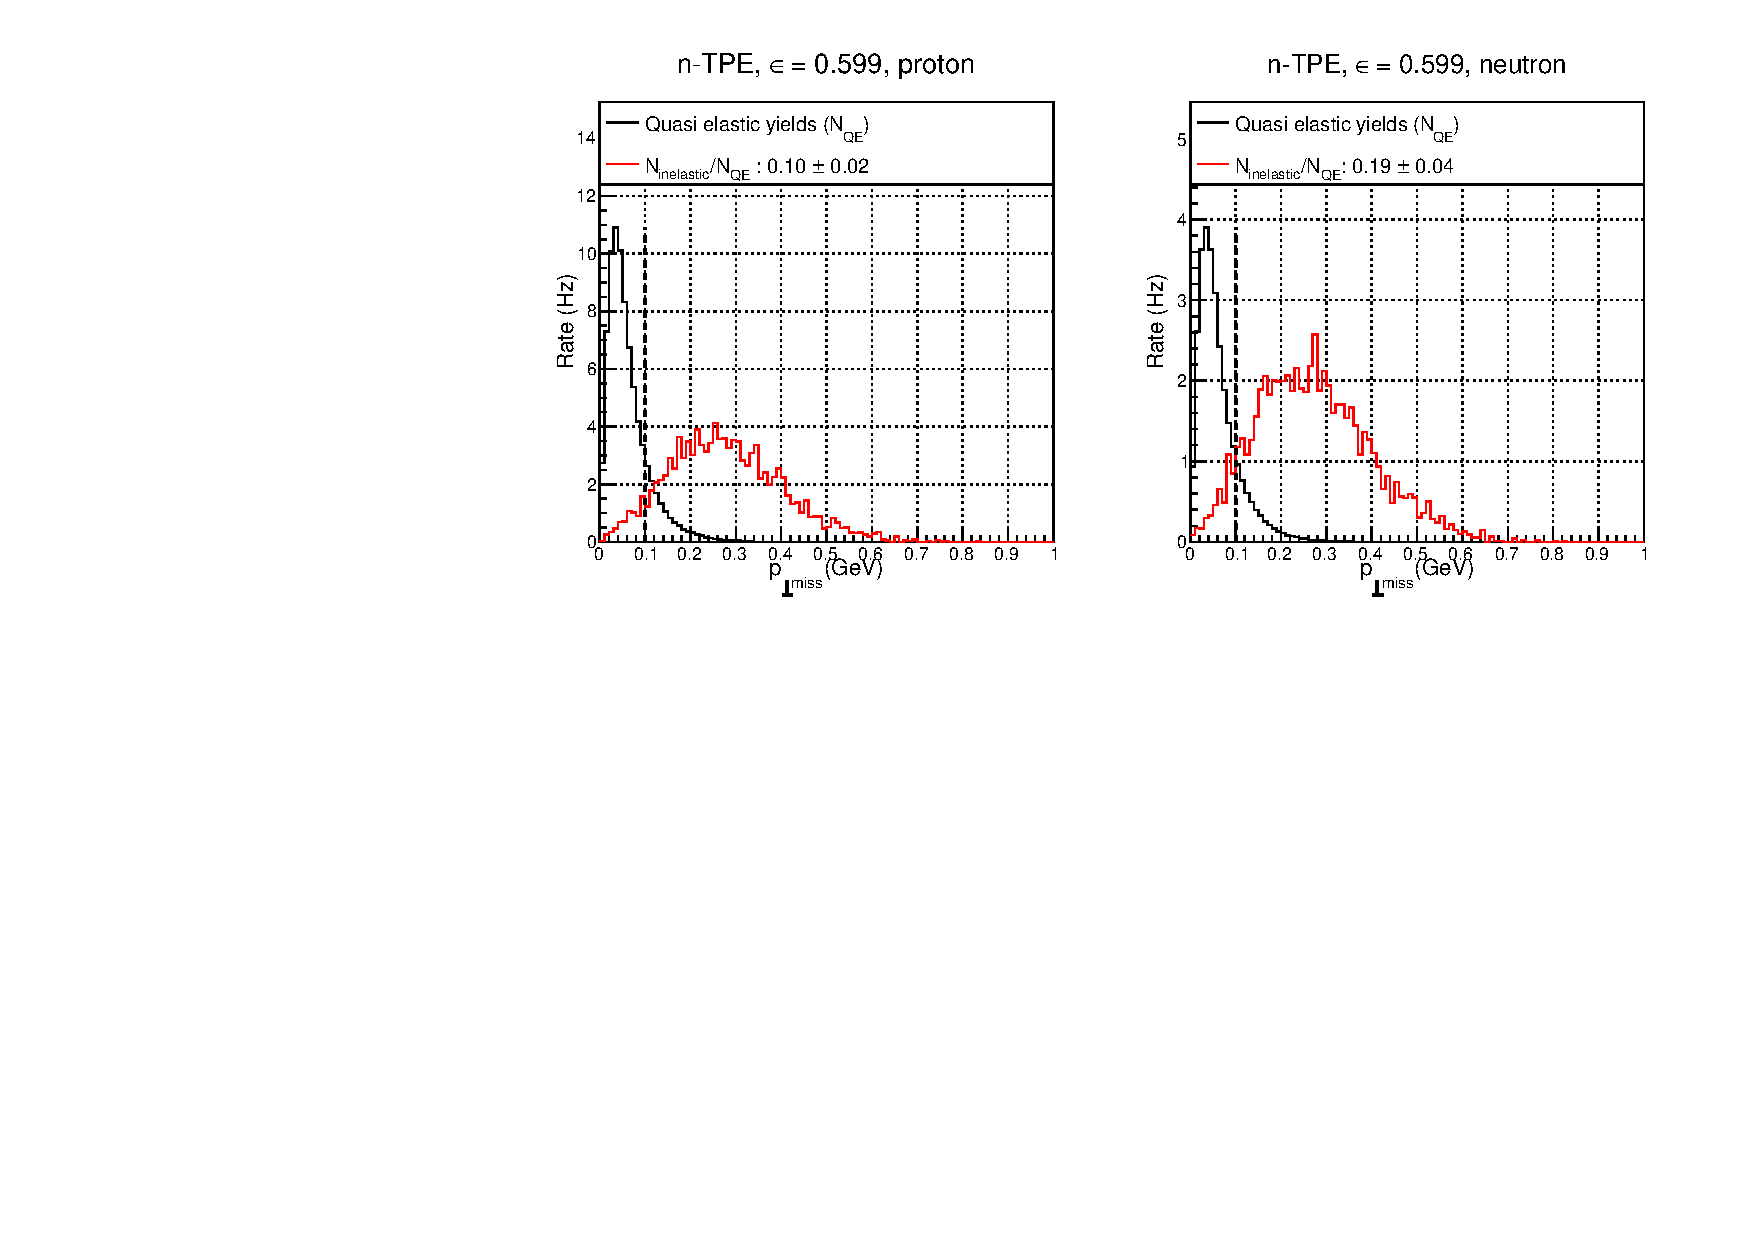
\includegraphics[width=12cm]{gen-tpe_le_pperp_acc_real.pdf}
    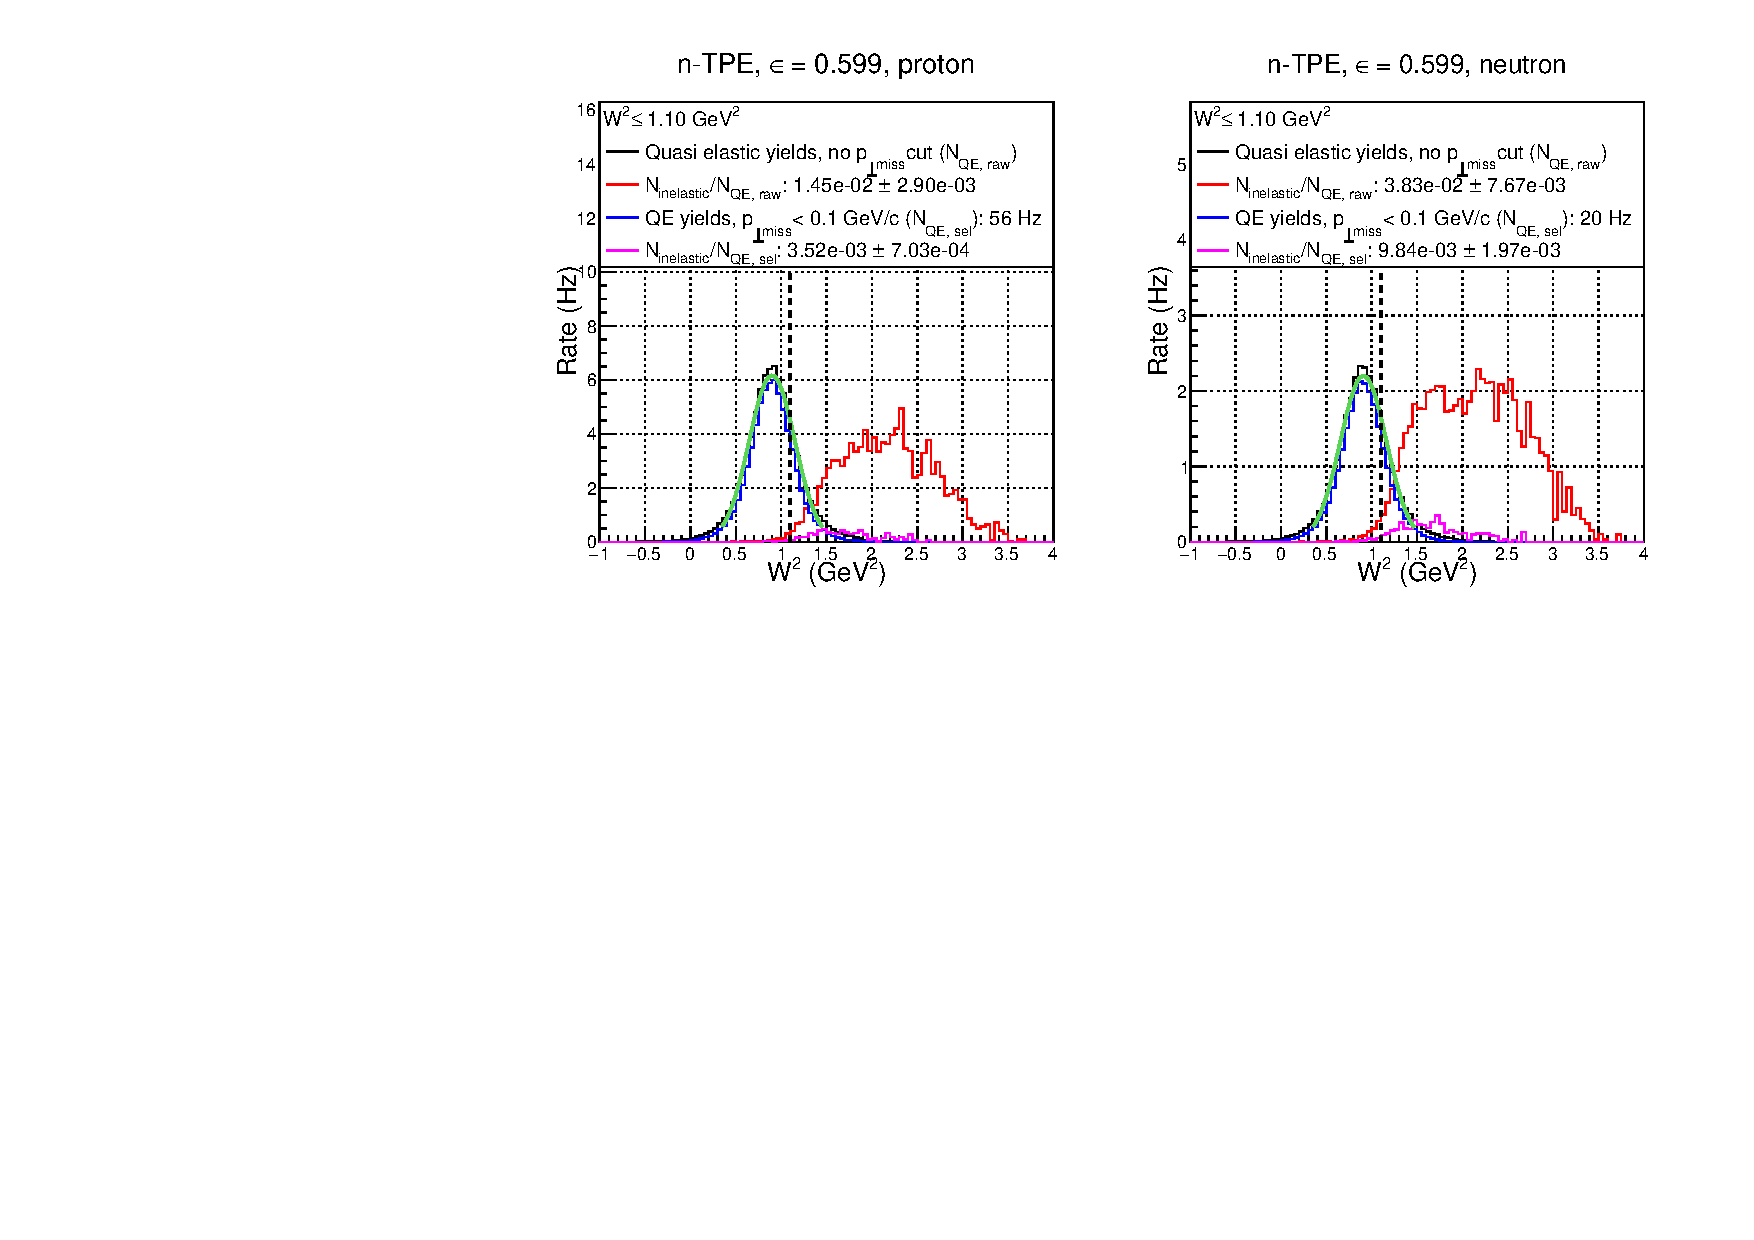
\includegraphics[width=12cm]{gen-tpe_le_W2_acc_real.pdf}
    \caption{Compared quasi-elastic and inelastic distributions (including detectors resolutions) for $p_{\perp miss} = \sqrt{(q_{x}-p'_{x})^2+(q_{y}-p'_{y})^2}$ (top) and $W^2 = M_{N}^2+2M_{N}^{2}(E-E')-Q^2$ (bottom), within fiducial analysis cuts, for the low $\epsilon$ kinematic. The inelastic contamination of quasi-elastic events and their error bars are quoted in the legends. Comparison for protons (resp. neutrons) is shown on the left (resp. on the right). On the bottom panel, black and red are before the $p_{\perp miss}~\leq~0.1~\mathrm{GeV}$ selection, while blue and magenta are after $p_{\perp miss}~\leq~0.1~\mathrm{GeV}$ selection.}
    \label{fig:inel_contam_le}
\end{figure}
%
\begin{figure}[h]
  \centering
    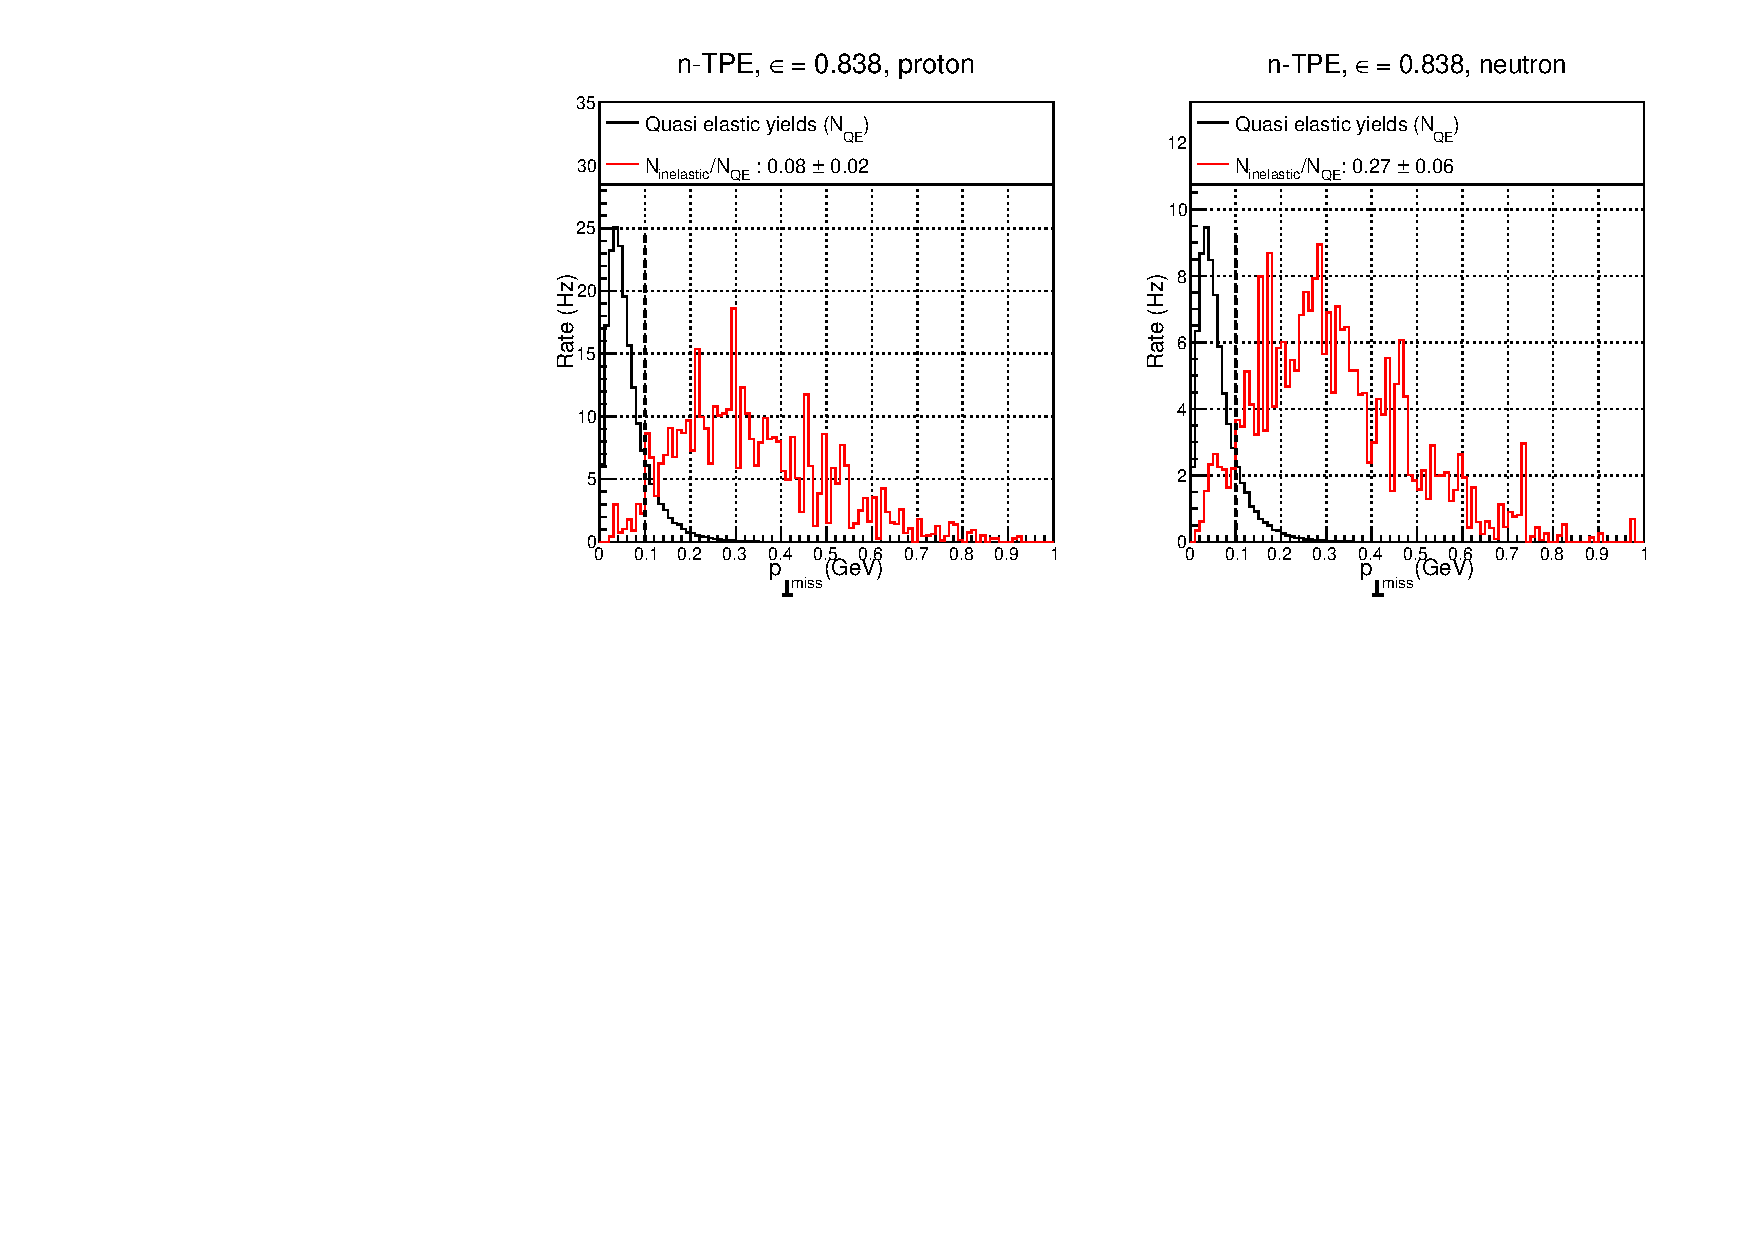
\includegraphics[width=12cm]{gen-tpe_he_pperp_acc_real.pdf}
    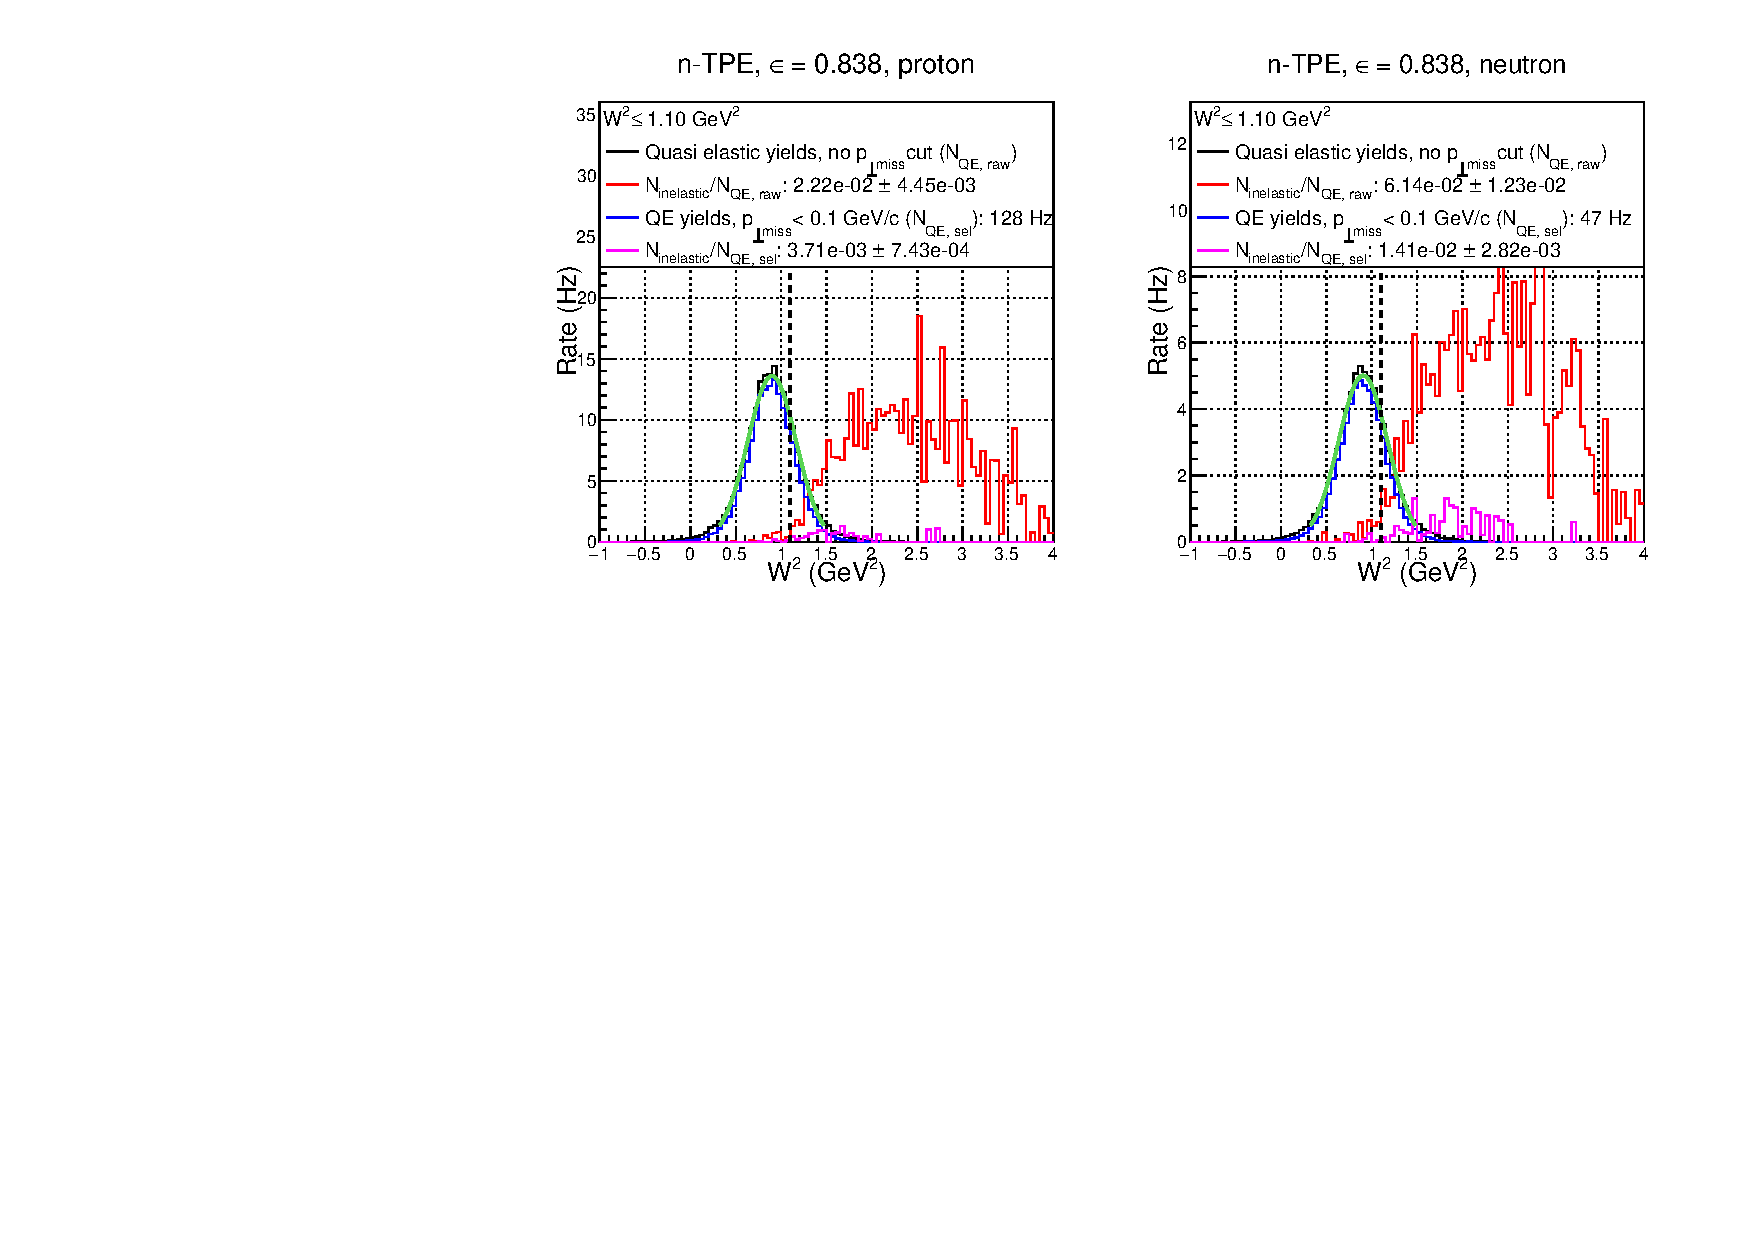
\includegraphics[width=12cm]{gen-tpe_he_W2_acc_real.pdf}
    \caption{Compared quasi-elastic and inelastic distributions (including detectors resolutions) for $p_{\perp miss} = \sqrt{(q_{x}-p'_{x})^2+(q_{y}-p'_{y})^2}$ (top) and $W^2 = M_{N}^2+2M_{N}^{2}(E-E')-Q^2$ (bottom), within fiducial analysis cuts, for the high $\epsilon$ kinematic. The inelastic contamination of quasi-elastic events and their error bars are quoted in the legends. Comparison for protons (resp. neutrons) is shown on the left (resp. on the right). On the bottom panel, black and red are before the $p_{\perp miss}~\leq~0.1~\mathrm{GeV}$ selection, while blue and magenta are after $p_{\perp miss}~\leq~0.1~\mathrm{GeV}$ selection and application of BigBite shower and HCal thresholds.}
    \label{fig:inel_contam_he}
\end{figure}
%

``The singles rate in HCal is huge and apparently the coincidence rate between BigBite and HCal is also large. How uncertain is the inelastic rate?''\\


``You base it on a model, how valid is it for your needs?''\\

%\comment{repeat ``This model is a fit of $e-N$ data in the resonance region...''?}
As stated earlier, this model is a fit of $e-N$ data in the resonance region from Jefferson Lab Hall C$^{3}$ which covers $0<=Q^2<8 {GeV/c}^2$, with beam energies up to 5.5 GeV.
It may be argued that provided the data set on which this fit is based (for which
the beam energy is no higher than 5.5 GeV),
we might use it at the limit of its validity for our high $\epsilon$ point (for which
the beam energy is 6.6 GeV).\\

``How much of the inelastic tail do you measure, e.g. how much of Figs. 10 and 11 will come from data?''\\

On figures~\ref{fig:inel_contam_le},~\ref{fig:inel_contam_he}, the red spectra are MC inelastic events detected in the BB/SBS coincidence, within our fiducial analysis cuts, in our simulation.
These are defined as:
%
\begin{itemize}
\item{a track passing through all GEM planes;}
\item{the total energy deposited in the Bigbite calorimeter above the threshold defined for this detector;}
\item{the track will fire at least 3 PMTs in the GRINCh detectors;}
\item{the total energy deposited in the hadron calorimeter is above the threshold defined for this detector.}
\end{itemize}
%

``If this background is twice as big as you expect, do you have recourse?''\\

If the background is dramatically larger than what we expect, we should be able to select in our data a clean inelastic sample.
We can use this inelastic sample to reevaluate our inelastic contamination prediction and subtract it.% The systematic uncertainty on the eN yield would be 20\% of the fraction of our new prediction.

We are confident that even if the inelastic background we observe is
dramatically higher than our prediction (say, even a factor 10), we have sufficient
leverage to understand this contamination and keep the uncertainty on the measured
en/ep ratios (and a fortiori on the Rosenbluth slope) under control. 
\fi

\paragraph{Question 4}
{\it Fig.2 might need more explanation. Apparently, you base your choice in
measurement scope and project uncertainty from it.}\\
{\it What uncertainties are in the results from Ref. 4 - both uncorrected and corrected?}\\
{\it Are these uncertainties included in your estimates?}\\
{\it Will you present your results in a way that theorists can do their own analysis?}\\

%\iffalse
``Fig.2 might need more explanation. Apparently, you base your choice in measurement scope and project uncertainty from it.''\\
The Fig.2 of the proposal, which was taken from Ref.4, used by us to estimate nTPE. However, it did not drive our choice in measurement, in part because there is a big uncertainty in
the calculations in Ref.4. Instead, we used information on proton TPE as a guidance on the $Q^2$ value to measure. For the proton we know that TPE become a dominant part of the Rosenbluth slope for $Q^2$ above 3 ${\rm(GeV/c)}^2$. 
The global fit on the proton Rosenbluth slope shown on Fig.1 of our proposal is an extension of the work done by J.~Arrington\footnote{Phys. Rev. C68, 034325 (2003), http://arxiv.org/abs/nucl-ex/0305009}, %~\cite{johna}, %
Fig.6 (reproduced here as figure~\ref{fig6refjohna})
%and A.~Puckett\footnote{Phys.~Rev.~C98, 019907 (2018), http://arxiv.org/abs/1102.5737}, %~\cite{andrew}, %
%Fig.3 (reproduced here as figure~\ref{fig3refandrew})
for lower $Q^2$.
The text of the GMp12 paper (draft) is attached.
All data points of Fig.1 of the proposal are from Table~I of the GMp12 paper draft (attached with the email).\\
%\fi

``What uncertainties are in the results from Ref. 4 - both uncorrected and corrected?''\\
Uncorrected data from Ref. 4 are based on a 1996 review\footnote{Nucl.~Phys.~A596, 367 (1996), http://arxiv.org/abs/hep-ph/9506375} %~\cite{drechsel}, %
which is now outdated. Actual value at $Q^2 =4.5~{\rm (GeV/c)}^2$ is a factor 2 larger than the prediction from review$^4$.
We base our analysis on a value for $\mu_n G_E^n/G_M^n$ from a 2015 review\footnote{Eur.~Phys.~J.~A51, (2015), http://arxiv.org/abs/1503.01452} %~\cite{ffrev},%
for which the uncertainty is about 10\%.\\
The uncertainty on the prediction of the neutron TPE contribution in Ref.4 of the proposal is indeed very large due to its model dependence. The numerical value of the uncertainty on the neutron TPE prediction is not specified in Ref.4.\\
It is large even for proton TPE, as it can be remarked from the growing error of the "corrected" data on Fig.5. of Ref.4, reproduced here on Figure~\ref{fig5ref4}.


``Are these uncertainties included in your estimates?''\\
The uncertainty on $\mu_n G_E^n/G_M^n$ %from\footnote{Eur.~Phys.~J.~A51, (2015), http://arxiv.org/abs/1503.01452}%\cite{ffrev}
is included in our estimate.
Not being explicitly specified, the uncertainty on the neutron TPE prediction from Ref.~4 is not included. We just use this prediction as a guidance for our projected value of the neutron Rosenbluth slope. We assumed that the ratio of the contributions of nTPE and $G_E^n$ to the Rosenbluth is the same as obtained in Ref.4. \\

``Will you present your results in a way that theorists can do their own analysis?''\\
We will produce publications providing the measured neutron slope, the nTPE contribution, and the cross sections at both $\epsilon$ values.

%
%\iffalse
\begin{figure}[!h]
  \begin{center}
    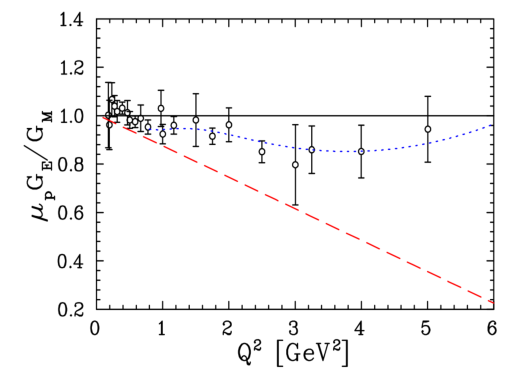
\includegraphics[width=8cm]{Fig6_refjohna.pdf}
    \caption{Ratio of electric to magnetic form factor as determined from direct Rosenbluth separations, using the normalizations determined from the global fit. %~\cite{johna}.
      The dotted line is the ratio from the global fit to $G_E^p$ and $G_M^p$, while the dashed line is the fit to the polarization measurements.
    Reproduced from Phys. Rev. C68, 034325 (2003), http://arxiv.org/abs/nucl-ex/0305009}
    \label{fig6refjohna}
  \end{center}
\end{figure}
%
%\begin{figure}[!h]
%  \begin{center}
%    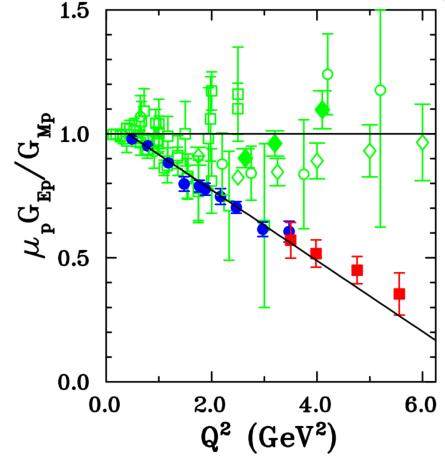
\includegraphics[width=8cm]{Papers/Fig3_refandrew.pdf}
%    \caption{The ratio $\mu_p G_E^p/G_M^p$ from the first two JLab experiments filled circle, and filled square, compared to  Rosenbluth  separation  results,  open  diamond,  open circle, filled diamond, and open square. The curve shows the linear fit to the polarization data. % from~\cite{PTdata}.
      %Reproduced from Phys. Rev. C68, 034325 (2003), http://arxiv.org/abs/nucl-ex/0305009
%    }
%    \label{fig3refandrew}
%  \end{center}
%\end{figure}
%\fi
%
\begin{figure}[!h]
  \begin{center}
    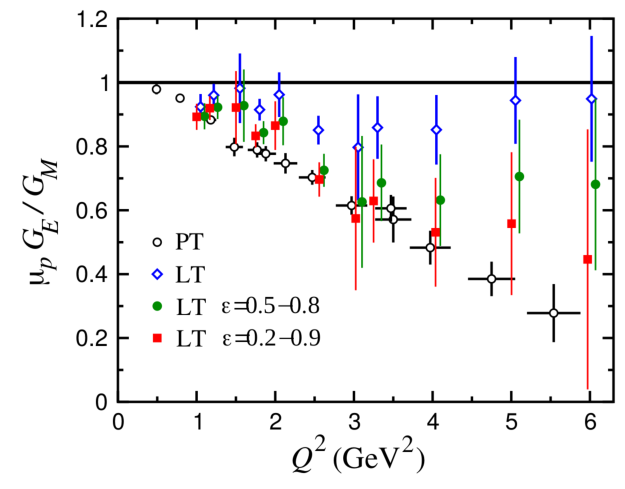
\includegraphics[width=8cm]{Fig5_ref4.pdf}
    \caption{The ratio of proton form factors $\mu_p G_E/G_M$ measured using Rosenbluth separation %~\cite{johna}
      (open diamonds, noted ``LT'' here) 
      and polarization transfer %~\cite{PTdata}
      (open circles, noted ``PT'' here). The ``LT'' points corrected for 2$\gamma$ exchange are
shown assuming a linear slope for $\epsilon$ = 0.2-0.9 (filled squares) and $\epsilon$ = 0.5-0.8 (filled circles)
(offset for clarity).
Reproduced from Ref.4 of the proposal.
    }
    \label{fig5ref4}
  \end{center}
\end{figure}
%



%
%\begin{equation}
%\end{equation}
%
%\begin{figure}[!h]
%  \begin{center}
%    \includegraphics[width=9.6cm,height=8cm]{Plots/EvtSizeGMn13.png}
%    \caption{}
%    \label{fig:evtsize}
%  \end{center}
%\end{figure}
%
%
%\begin{itemize}
%\item{}
%\end{itemize}
%
    

\iffalse
\begin{thebibliography}{9}
\bibitem{PRL}{G.D.~Cates, C.W.~de~Jager, S.~Riordan, B.~Wojtsekhowski, Phys.~Rev.~Lett.~106, 252003 (2011),\\ http://arxiv.org/abs/1103.1808 }%, \hyperlink{http://arxiv.org/pdf/1103.1808.pdf}{arxiv:1103.1808}}http://arxiv.org/abs/1103.1808
\bibitem{johna}{J.~Arrington, Phys. Rev. C68, 034325 (2003),\\ http://arxiv.org/abs/nucl-ex/0305009 }%, \hyperlink{http://arxiv.org/pdf/nucl-ex/0305009.pdf}{arxiv:nucl-ex/0305009}}http://arxiv.org/abs/nucl-ex/0305009
\bibitem{andrew}{A.~Puckett {\it et~al.}, Phys.~Rev.~C98, 019907 (2018), http://arxiv.org/abs/1102.5737 }%, \hyperlink{http://arxiv.org/pdf/1102.5737.pdf}{arxiv:1102.5737}}
\bibitem{PTdata}{M.~K.~Jones {\it et~al.}, Phys.~Rev.~Lett.~84, 1398 (2000),\\ http://arxiv.org/abs/nucl-ex/9910005 ;\\ %, \hyperlink{http://arxiv.org/pdf/nucl-ex/9910005.pdf}{arxiv:nucl-ex/9910005};
  O.~Gayou {\it et~al.}, Phys.~Rev.~Lett.~88, 092301 (2002),\\ http://arxiv.org/abs/nucl-ex/0111010 ;\\%, \hyperlink{http://arxiv.org/pdf/nucl-ex/0111010.pdf}{arxiv:nucl-ex/0111010};http://arxiv.org/abs/nucl-ex/0111010
  V.~Punjabi {\it et~al.},\\ http://arxiv.org/abs/nucl-ex/0501018.}% \hyperlink{http://arxiv.org/pdf/nucl-ex/0501018.pdf}{arxiv:nucl-ex/0501018.}}
\bibitem{drechsel}{P.~Mergell, U.~G.~Meissner, and D.~Drechsel, Nucl.~Phys.~A596, 367 (1996), \\ http://arxiv.org/abs/hep-ph/9506375 }
\bibitem{ffrev}{V.~Punjabi, C.~F.~Perdrisat, M.~K.~Jones, E.~J.~Brash, and C.~E.~Carlson, Eur.~Phys.~J.~A51, (2015), \\ http://arxiv.org/abs/1503.01452 }
\end{thebibliography}
\fi
\end{document}
